% !TEX encoding = UTF-8
% !TEX program = pdflatex
\documentclass[a4paper,titlepage,11pt,floatssmall]{mwrep}
\usepackage[left=2.5cm,right=2.5cm,top=2.5cm,bottom=2.5cm]{geometry}
\usepackage[T1]{fontenc}
\usepackage{lmodern}
\usepackage[utf8]{inputenc}
\usepackage{polski}
\usepackage{amsmath,amssymb}
\usepackage{graphicx,float,booktabs,array}
\usepackage{xcolor,listings}
\usepackage{siunitx}
\sisetup{output-decimal-marker={,},group-separator={\,},group-minimum-digits=5,group-digits=integer}
\usepackage[hidelinks,unicode]{hyperref}
\hypersetup{pdftitle={Sztuczna Inteligencja w Automatyce -- części 1--3: układ zbiorników},pdfauthor={Mikołaj Wróbel, Wojciech Zieliński},pdfsubject={Projekt, semestr zimowy 2026/2027}}
\definecolor{szary}{rgb}{0.96,0.96,0.96}
\lstdefinestyle{custommatlab}{language=Matlab,basicstyle=\footnotesize\ttfamily,
  backgroundcolor=\color{szary},frame=single,breaklines=true,
  showstringspaces=false,keywordstyle=\color{blue!60!black},
  commentstyle=\color{green!35!black},columns=fullflexible}
\renewcommand{\figurename}{Rys.}
\renewcommand{\tablename}{Tab.}
\newcommand{\jednprzep}{\mathrm{cm^3/s}}
\newcommand{\uop}{F_{1\mathrm{in},0}}
\newcommand{\uvar}{F_{1\mathrm{in}}}
% Wczytywanie wierszy tabel bez haków plikowych wewnątrz tabular.
\makeatletter
\let\tableinput\@@input
\makeatother
\setcounter{topnumber}{3}
\setcounter{bottomnumber}{2}
\setcounter{totalnumber}{5}
\renewcommand{\textfraction}{0.08}
\renewcommand{\topfraction}{0.92}
\renewcommand{\bottomfraction}{0.85}
\renewcommand{\floatpagefraction}{0.65}
\begin{document}
\frenchspacing
\raggedbottom
\setlength{\intextsep}{8pt}
\pagestyle{uheadings}
\hypersetup{pageanchor=false}
\begin{titlepage}
\begin{center}
{\LARGE\bfseries Politechnika Warszawska\par}
\vspace{0.4cm}
{\Large Wydział Elektroniki i Technik Informacyjnych\par}
\vspace{3.3cm}
{\LARGE\bfseries Sztuczna Inteligencja w Automatyce\par}
\vspace{0.7cm}
{\Large Projekt -- semestr zimowy 2026/2027\par}
\vspace{1.2cm}
{\LARGE\bfseries Sprawozdanie -- części 1--3\par}
\vspace{0.6cm}
{\Large Układ zbiorników (zadanie 1)\par}
\vspace{0.4cm}
{\large Model nieliniowy i liniowy, modele Takagiego--Sugeno\par
oraz analityczny i numeryczny rozmyty regulator DMC\par}
\vspace{2cm}
{\large Mikołaj Wróbel, nr indeksu 337021\par}
\vspace{0.4cm}
{\large Wojciech Zieliński, nr indeksu 337000\par}
\vfill
{\large Warszawa, 2026\par}
\end{center}
\end{titlepage}
\hypersetup{pageanchor=true}
\pagenumbering{arabic}
\chapter{Model obiektu}
Zbadano odpowiedzi układu dwóch zbiorników, wyznaczono model liniowy w punkcie pracy i sprawdzono działanie konwencjonalnego regulatora DMC. Wyjściem jest poziom $h_2$, sterowaniem dopływ $\uvar$, a zakłóceniem dopływ $F_D$.

\section{Model nieliniowy i punkt pracy}
Model opisują bilanse objętości oraz zależności geometryczne:
\begin{align}
\dot V_1&=\uvar(t-\tau)+F_D-\alpha_1\sqrt{h_1},\\
\dot V_2&=\alpha_1\sqrt{h_1}-\alpha_2\sqrt{h_2},\\
V_1&=A_1h_1,\qquad V_2=C_2h_2^3.
\end{align}
Przyjęto $A_1=560\ \mathrm{cm^2}$, $C_2=\num{0.6}$, $\alpha_1=29$, $\alpha_2=33$ oraz $\tau=200\ \mathrm{s}$. W punkcie pracy $\uop=100\ \jednprzep$ i $F_{D,0}=20\ \jednprzep$. Warunek równowagi daje
\begin{equation}
h_{1,0}=\left(\frac{120}{29}\right)^2\approx\num{17.1225}\ \mathrm{cm},\qquad
h_{2,0}=\left(\frac{120}{33}\right)^2\approx\num{13.2231}\ \mathrm{cm}.
\end{equation}
Wszystkie próby rozpoczynano od tego samego punktu równowagi. Zastosowano okres próbkowania $T_s=20\ \mathrm{s}$; opóźnienie sterowania odpowiada 10 próbkom. Zakłócenie $F_D$ działa bez tego opóźnienia.

\section{Model liniowy}
Zlinearyzowano równania względem poziomów w punkcie pracy. Dla $x=[\Delta h_1,\Delta h_2]^{\mathsf T}$ otrzymano
\begin{equation}
\dot x=
\begin{bmatrix}-\num{0.00625744}&0\\\num{0.01113379}&-\num{0.01441700}\end{bmatrix}x+
\begin{bmatrix}1/560&1/560\\0&0\end{bmatrix}
\begin{bmatrix}\Delta u(t-200)\\\Delta d(t)\end{bmatrix},\quad
\Delta y=\begin{bmatrix}0&1\end{bmatrix}x,
\end{equation}
gdzie $\Delta u=\uvar-100$, $\Delta d=F_D-20$ oraz $\Delta y=h_2-h_{2,0}$. Transmitancje mają postać
\begin{equation}
G_u(s)=\frac{\num{0.220386}\,e^{-200s}}{(\num{159.81}s+1)(\num{69.36}s+1)},\qquad
G_d(s)=G_u(s)e^{200s}.
\end{equation}
Model liniowy ma dwie inercje i dodatnie wzmocnienie statyczne. Różnica między torami sterowania i zakłócenia polega na opóźnieniu.

\chapter{Porównanie modeli}
Porównano odpowiedzi obu modeli na skoki wejść do $\pm50\%$ wartości nominalnych. Każda próba rozpoczyna się od podanego punktu równowagi.

\section{Tor sterowania}
\begin{figure}[H]
\centering
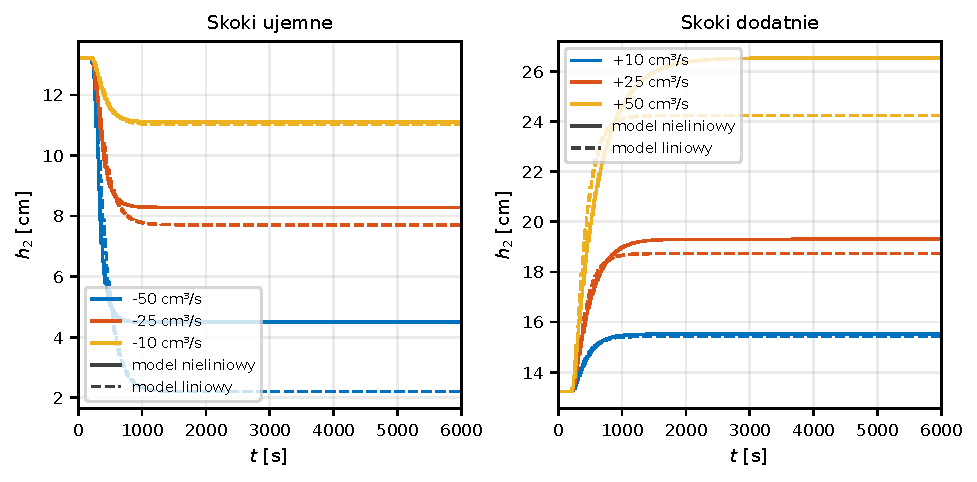
\includegraphics[width=0.90\textwidth]{rysunki/czesc1/skoki_F1in.pdf}
\caption{Skoki sterowania o $\pm10$, $\pm25$ i $\pm50\ \jednprzep$ przy stałym $F_D=20\ \jednprzep$.}
\label{fig:skokiU}
\end{figure}
Blisko punktu pracy odpowiedzi są zbliżone. Dla większych skoków różnią się poziom końcowy i szybkość zmian. Błąd statyczny dla skoków $\pm10\ \jednprzep$ wynosi około $\num{0.092}\ \mathrm{cm}$, a dla $\pm50\ \jednprzep$ około $\num{2.30}\ \mathrm{cm}$.

\section{Tor zakłócenia}
\begin{figure}[H]
\centering
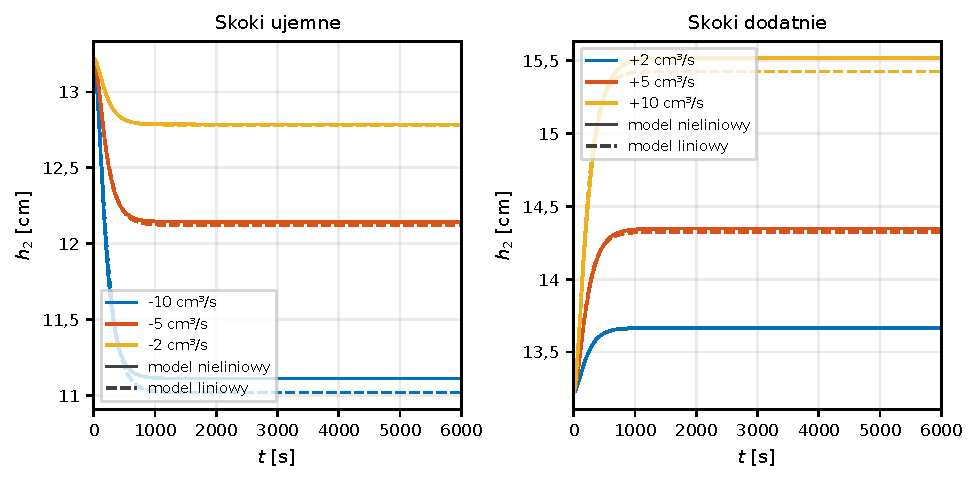
\includegraphics[width=0.90\textwidth]{rysunki/czesc1/skoki_FD.pdf}
\caption{Skoki zakłócenia o $\pm2$, $\pm5$ i $\pm10\ \jednprzep$ przy stałym $\uvar=100\ \jednprzep$.}
\label{fig:skokiD}
\end{figure}
Zakłócenie działa bez opóźnienia transportowego. Różnice modeli są mniejsze, ponieważ skoki $F_D$ mają mniejsze amplitudy bezwzględne niż skoki sterowania.

\chapter{Regulacja DMC}
\section{Algorytm i testy}
Zaprojektowano analityczny regulator DMC na podstawie odpowiedzi skokowej modelu liniowego. W każdej próbce algorytm wyznacza przyszłe przyrosty sterowania minimalizujące błąd predykcji wyjścia i zmiany sterowania, a na obiekt podaje tylko pierwszy z nich. Dzięki uwzględnieniu historii sterowań regulator dobrze radzi sobie z opóźnieniem transportowym $200\ \mathrm{s}$. Przyjęto nastawy: $D=250$, $N=50$, $N_u=10$, $\lambda=\num{0.05}$ oraz $T_s=20\ \mathrm{s}$. Regulator działa bez ograniczeń, a zakłócenie $F_D$ tłumi przez sprzężenie zwrotne.

Na obu obiektach w $400\ \mathrm{s}$ zmieniano zadany poziom, a w $3800\ \mathrm{s}$ zakłócenie. Dla każdej próby pokazano wyjście $y(k)=h_2(k)$ i sterowanie $u(k)=\uvar(k)$ na wspólnej osi czasu.
\begin{figure}[H]
\centering
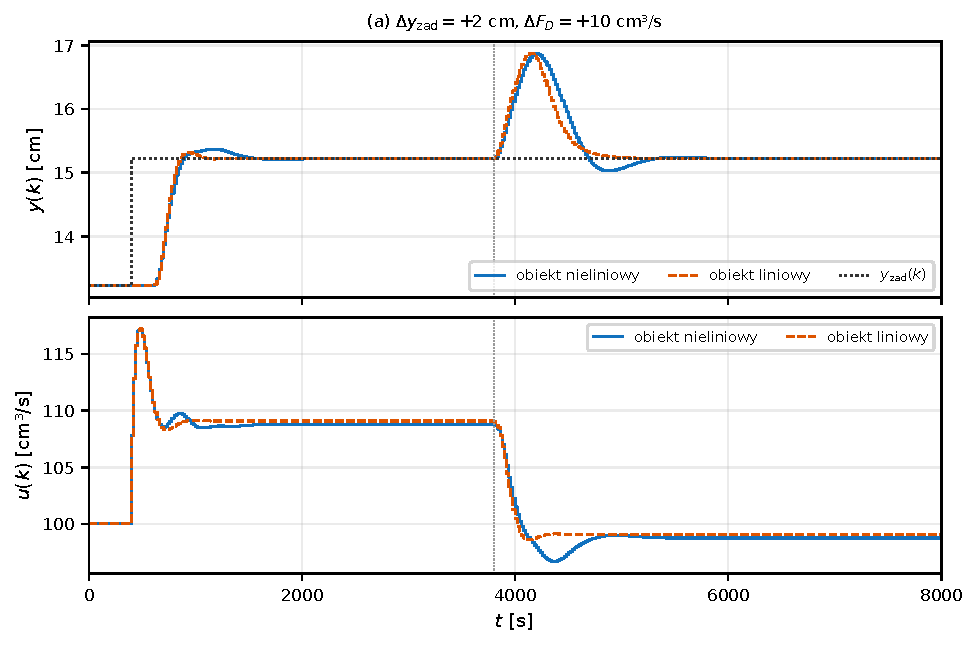
\includegraphics[width=0.94\textwidth]{rysunki/czesc1/DMC_scenariusz_1.pdf}
\caption{Próba 1: $\Delta y_{\mathrm{zad}}=+2\ \mathrm{cm}$, $\Delta F_D=+10\ \jednprzep$. Wyjście $y(k)$ i bezpośrednio pod nim sterowanie $u(k)$; pionowa linia oznacza skok $F_D$.}
\label{fig:dmcY}
\end{figure}
Dla małych skoków przebiegi obu obiektów są zbliżone, zarówno dla wyjścia, jak i sterowania.

\clearpage
\section{Skok zadania o 4 cm}
Po dodatnim skoku zakłócenia regulator zmniejsza dopływ. Skutek korekcji dociera do obiektu po czasie transportu, dlatego poziom przejściowo rośnie.
\begin{figure}[H]
\centering
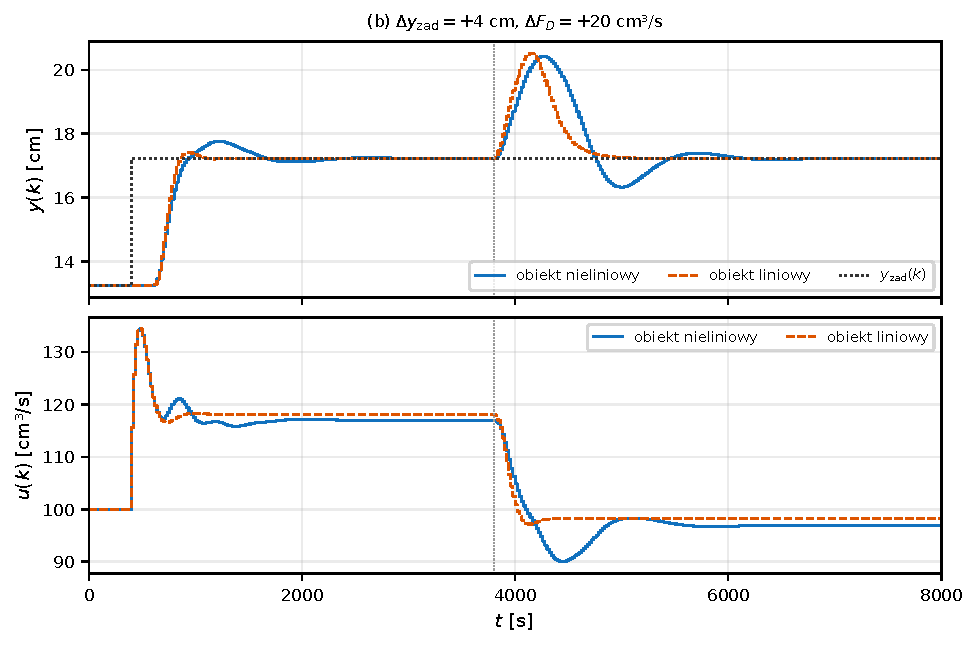
\includegraphics[width=0.94\textwidth]{rysunki/czesc1/DMC_scenariusz_2.pdf}
\caption{Próba 2: $\Delta y_{\mathrm{zad}}=+4\ \mathrm{cm}$, $\Delta F_D=+20\ \jednprzep$. Wyjście i sterowanie na wspólnej osi czasu.}
\label{fig:dmcU}
\end{figure}

\clearpage
\section{Duży dodatni skok zadania}
\begin{figure}[H]
\centering
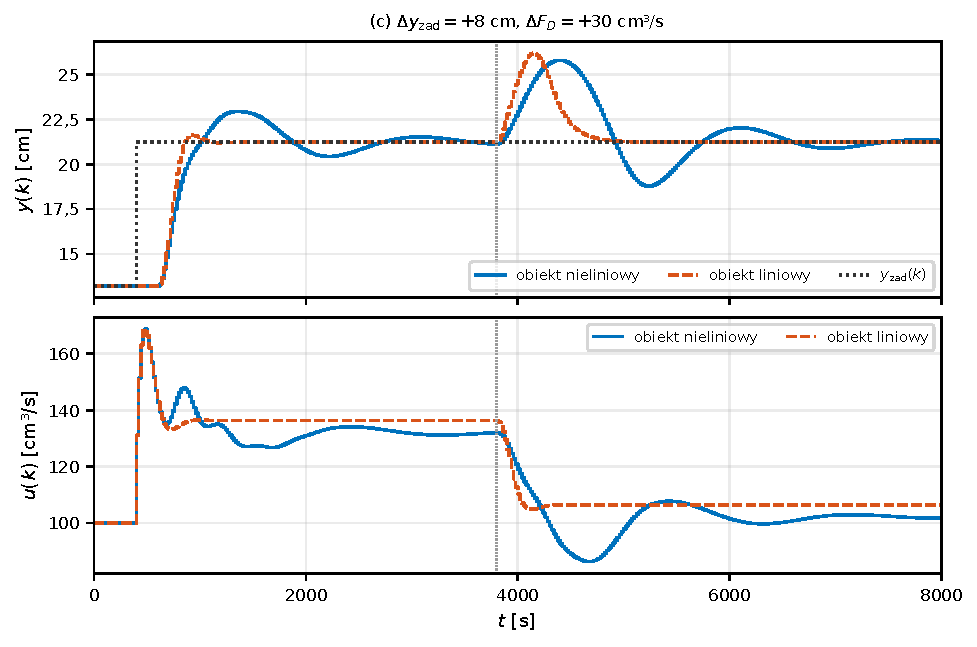
\includegraphics[width=\textwidth]{rysunki/czesc1/DMC_scenariusz_3.pdf}
\caption{Próba 3: $\Delta y_{\mathrm{zad}}=+8\ \mathrm{cm}$, $\Delta F_D=+30\ \jednprzep$. Wyjście $y(k)$ oraz odpowiadające mu sterowanie $u(k)$.}
\label{fig:dmc4}
\end{figure}
Przy dużym dodatnim skoku obiekt nieliniowy silniej oscyluje. Widać również większe korekty sterowania niż dla obiektu liniowego. Maksymalna różnica wyjść sięga $\num{3.37}\ \mathrm{cm}$.

\clearpage
\section{Duży ujemny skok zadania}
\begin{figure}[H]
\centering
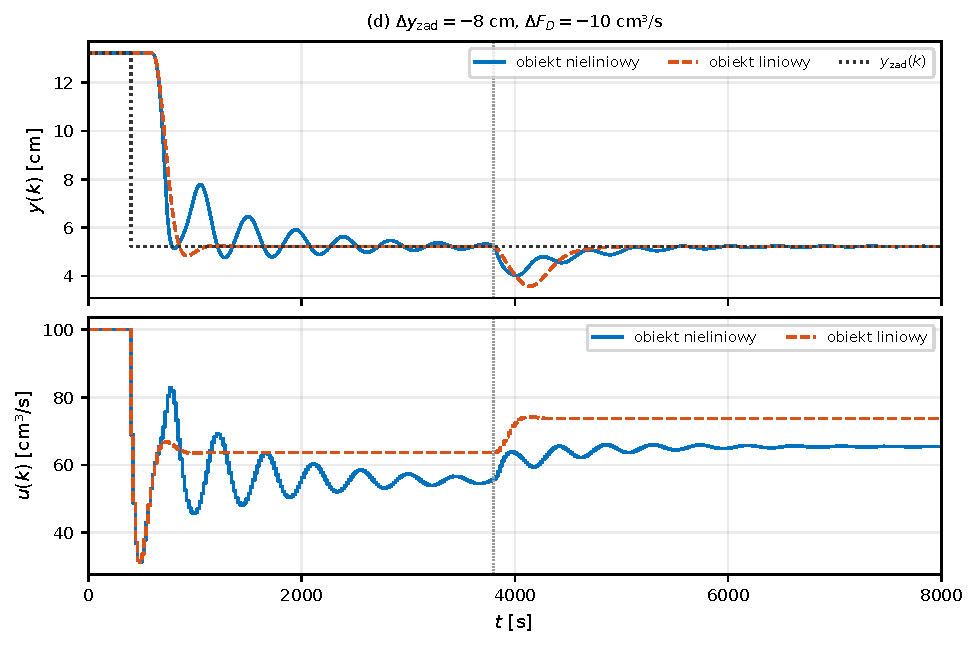
\includegraphics[width=\textwidth]{rysunki/czesc1/DMC_scenariusz_4.pdf}
\caption{Próba 4: $\Delta y_{\mathrm{zad}}=-8\ \mathrm{cm}$, $\Delta F_D=-10\ \jednprzep$. Wyjście $y(k)$ i sterowanie $u(k)$.}
\label{fig:dmcUjemny}
\end{figure}
Obniżenie zadania wymaga zmniejszenia dopływu. Oscylacje poziomu na obiekcie nieliniowym wiążą się z oscylacjami sterowania. Minimalny dopływ to około $\num{31.19}\ \jednprzep$.

\clearpage
\section{Ocena jakości regulacji}
Uchyb regulacji to wartość zadana $y_{\mathrm{zad}}(k)$ minus zmierzony poziom $y(k)=h_2(k)$:
\begin{equation}
e(k)=y_{\mathrm{zad}}(k)-y(k).
\end{equation}
Jakość regulacji obiektu nieliniowego oceniono wskaźnikiem
\begin{equation}
\mathrm{IAE}=T_s\sum_k|y_{\mathrm{zad}}(k)-y(k)|=T_s\sum_k|e(k)|.
\end{equation}
Dla zadania sumowano próbki od $400$ do chwili poprzedzającej $3800\ \mathrm{s}$, a dla zakłócenia od $3800$ do $8000\ \mathrm{s}$.
\begin{table}[H]
\centering\small
\caption{Wyniki regulacji obiektu nieliniowego i różnica wyjść obu pętli}
\begin{tabular}{rrrrr}
\toprule
$\Delta y_{\mathrm{zad}}$ & $\Delta F_D$ & $\mathrm{IAE}_{\mathrm{zad}}$ & $\mathrm{IAE}_D$ & $\max|y_{\mathrm{NL}}-y_{\mathrm{L}}|$\\
{}[cm] & [$\jednprzep$] & [$\mathrm{cm\cdot s}$] & [$\mathrm{cm\cdot s}$] & [cm]\\
\midrule
\tableinput{dane/DMC_wskazniki.tex}
\bottomrule
\end{tabular}
\end{table}
W badanych próbach sterowanie pozostało dodatnie; najmniejsza wartość wynosiła około $\num{31.19}\ \jednprzep$. Przy większych skokach rosną oscylacje i rozbieżności modeli. W dodatnich scenariuszach zwiększano jednocześnie zmianę zadania i zakłócenia, dlatego sam wzrost IAE nie pozwala oddzielić wpływu tych dwóch czynników.

\section{Wnioski}
\begin{itemize}
\item Model liniowy dobrze przybliża obiekt w pobliżu punktu pracy. Przy dużych zmianach dopływu błędy poziomu i dynamiki stają się wyraźne.
\item DMC uwzględnia opóźnienie i zapewnia śledzenie zadania oraz tłumienie zakłóceń w badanych próbach. Przy zmianach zadania o $\pm8\ \mathrm{cm}$ odpowiedź nieliniowa jest bardziej oscylacyjna.
\item Jeden model lokalny nie opisuje równie dobrze całego zakresu pracy. Wyniki stanowią punkt odniesienia dla regulatorów rozmytych w dalszych częściach projektu.
\end{itemize}
\smallskip
{\small Źródła: treść zadania \texttt{main (50).pdf}, część 1; skrypt \texttt{run\_part1.m}.}

\chapter{Modele rozmyte Takagiego--Sugeno}
\section{Zmienna reguł i dyskretne modele lokalne}
Zmienną przesłanek jest poziom $h_2$, od którego zależy przekrój drugiego zbiornika $B_2(h_2)=3C_2h_2^2$ oraz reakcja układu na niemierzalne zakłócenie $F_D$. Zakres $h_2\in[\num{4.500},\ \num{26.538}]\ \mathrm{cm}$ odpowiada zmianom dopływu $\uvar$ od 50 do 150~$\jednprzep$ ($\pm50\%$) przy $F_{D,0}=20\ \jednprzep$. Podzielono go równomiernie na 2, 3, 4 i 5~węzłów z trójkątnymi funkcjami przynależności (z ramionami na brzegach), sumującymi się do jedności.

W każdym węźle $h_{2,i}$ wyznaczono punkt równowagi $q_i=\alpha_2\sqrt{h_{2,i}}$, $h_{1,i}=(q_i/\alpha_1)^2$ oraz linearyzację obiektu:
\begin{align}
\dot h &= A_i(h-h_i)+B\bigl(\uvar(t-\tau)+F_D(t)-q_i\bigr),\\
A_i&=\begin{bmatrix}-k_{1,i}/A_1&0\\k_{1,i}/B_{2,i}&-k_{2,i}/B_{2,i}\end{bmatrix},\quad
B=\begin{bmatrix}1/A_1\\0\end{bmatrix},\\
k_{1,i}&=\frac{\alpha_1}{2\sqrt{h_{1,i}}},\quad
k_{2,i}=\frac{\alpha_2}{2\sqrt{h_{2,i}}},\quad B_{2,i}=3C_2h_{2,i}^2.
\end{align}
Modele lokalne zdyskretyzowano metodą ZOH (\texttt{c2d}, $T_s=20\ \mathrm{s}$) do równań różnicowych (materiały wykładowe \emph{Modele rozmyte}, s.~133--134, wzory (4.38) i (4.41)):
\begin{align}
 y^i(k+1)&=b_{1,i}\,y(k)+b_{2,i}\,y(k-1)+c_{1,i}\,q(k)+c_{2,i}\,q(k-1)+a_{0,i}^q,\\
 y(k+1)&=\sum_{i=1}^r\widetilde w_i\bigl(y(k)\bigr)\,y^i(k+1),\qquad
 \widetilde w_i(h_2)=\frac{\mu_i(h_2)}{\sum_{\ell=1}^r\mu_\ell(h_2)},
\end{align}
gdzie $q(k)=\uvar(k-10)+F_D(k)$ oraz $a_{0,i}^q=(1-b_{1,i}-b_{2,i})h_{2,i}-(c_{1,i}+c_{2,i})q_i$. W modelach używanych przez regulatory zakłada się nominalne $F_D=F_{D,0}=20\ \jednprzep$, co daje $y^i(k+1)=b_{1,i}y(k)+b_{2,i}y(k-1)+c_{1,i}u(k-10)+c_{2,i}u(k-11)+a_{0,i}$ dla $a_{0,i}=(1-b_{1,i}-b_{2,i})h_{2,i}-(c_{1,i}+c_{2,i})(q_i-F_{D,0})$. Próby rozpoczynano w nominalnym punkcie pracy $h_{2,0}\approx\num{13.223}\ \mathrm{cm}$.

\begin{figure}[H]
\centering
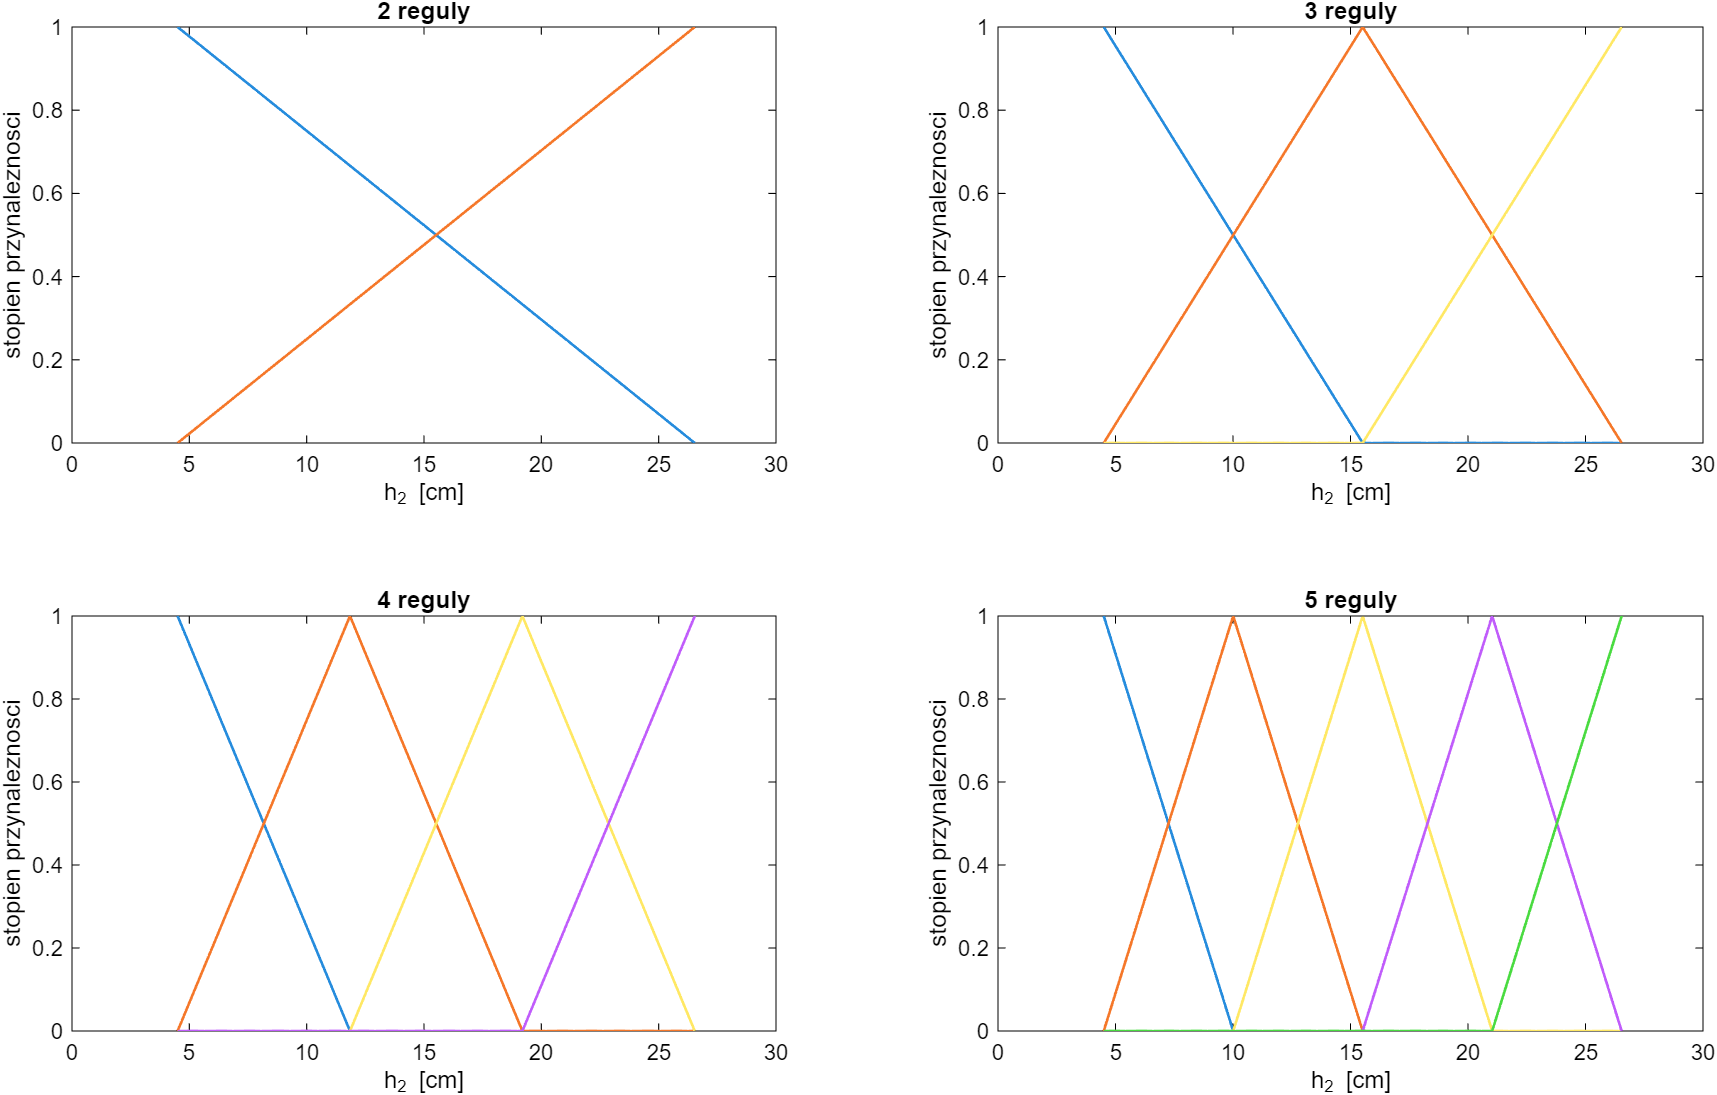
\includegraphics[width=0.92\textwidth]{rysunki/czesc2/funkcje_przynaleznosci.png}
\caption{Początkowe funkcje przynależności dla 2--5 reguł.}
\label{fig:ts-mf}
\end{figure}

\section{Porównanie jakości modeli}
Modele sprawdzono na 12 skokach z punktu pracy ($\Delta\uvar=\pm10,\pm25,\pm50\ \jednprzep$ oraz $\Delta F_D=\pm2,\pm5,\pm10\ \jednprzep$) w czasie $6000\ \mathrm{s}$. Błąd RMSE liczono względem obiektu nieliniowego po wszystkich próbkach; odniesieniem jest model liniowy z części~1.
\begin{table}[H]
\centering
\caption{Jakość modeli na 12 skokach z punktu pracy (przed strojeniem).}
\begin{tabular}{lrr}\toprule
Model & RMSE [cm] & Maksymalny błąd [cm]\\\midrule
Liniowy & \num{0.878} & \num{2.296}\\
TS, 2 reguły & \num{3.369} & \num{8.895}\\
TS, 3 reguły & \num{1.615} & \num{2.442}\\
TS, 4 reguły & \num{0.393} & \num{1.499}\\
TS, 5 reguł & \num{0.207} & \num{1.457}\\\bottomrule
\end{tabular}
\label{tab:ts-quality}
\end{table}

Dla 2 i 3 reguł uśrednianie szeroko rozstawionych linearyzacji przesuwa punkt równowagi modelu względem $h_{2,0}$ (widoczne już w pierwszych 200~s na rys.~\ref{fig:ts-models}). Od czterech reguł błąd spada poniżej modelu liniowego, a przy pięciu regułach RMSE osiąga \num{0.207}~cm -- ten model wybrano do dalszych badań. W tab.~\ref{tab:ts-amplitude} rozbito RMSE według amplitudy skoków obu wejść.

\begin{table}[H]
\centering
\caption{RMSE poziomu $h_2$ [cm] w zależności od amplitudy skoku.}
\small
\begin{tabular}{crrrrrr}\toprule
Amplituda & Liniowy & TS 2 & TS 3 & TS 4 & TS 5 & TS 5 strojony\\\midrule
10\% & \num{0.060} & \num{2.384} & \num{1.947} & \num{0.408} & \num{0.132} & \num{0.105}\\
25\% & \num{0.373} & \num{2.937} & \num{1.447} & \num{0.269} & \num{0.237} & \num{0.101}\\
50\% & \num{1.472} & \num{4.442} & \num{1.394} & \num{0.474} & \num{0.235} & \num{0.190}\\\bottomrule
\end{tabular}
\label{tab:ts-amplitude}
\end{table}

Dla małych skoków 10\% najdokładniejszy pozostaje model liniowy w punkcie pracy, natomiast przy zmianach 25\% i 50\% wyraźnie lepiej wypada model TS 5.

\begin{figure}[H]
\centering
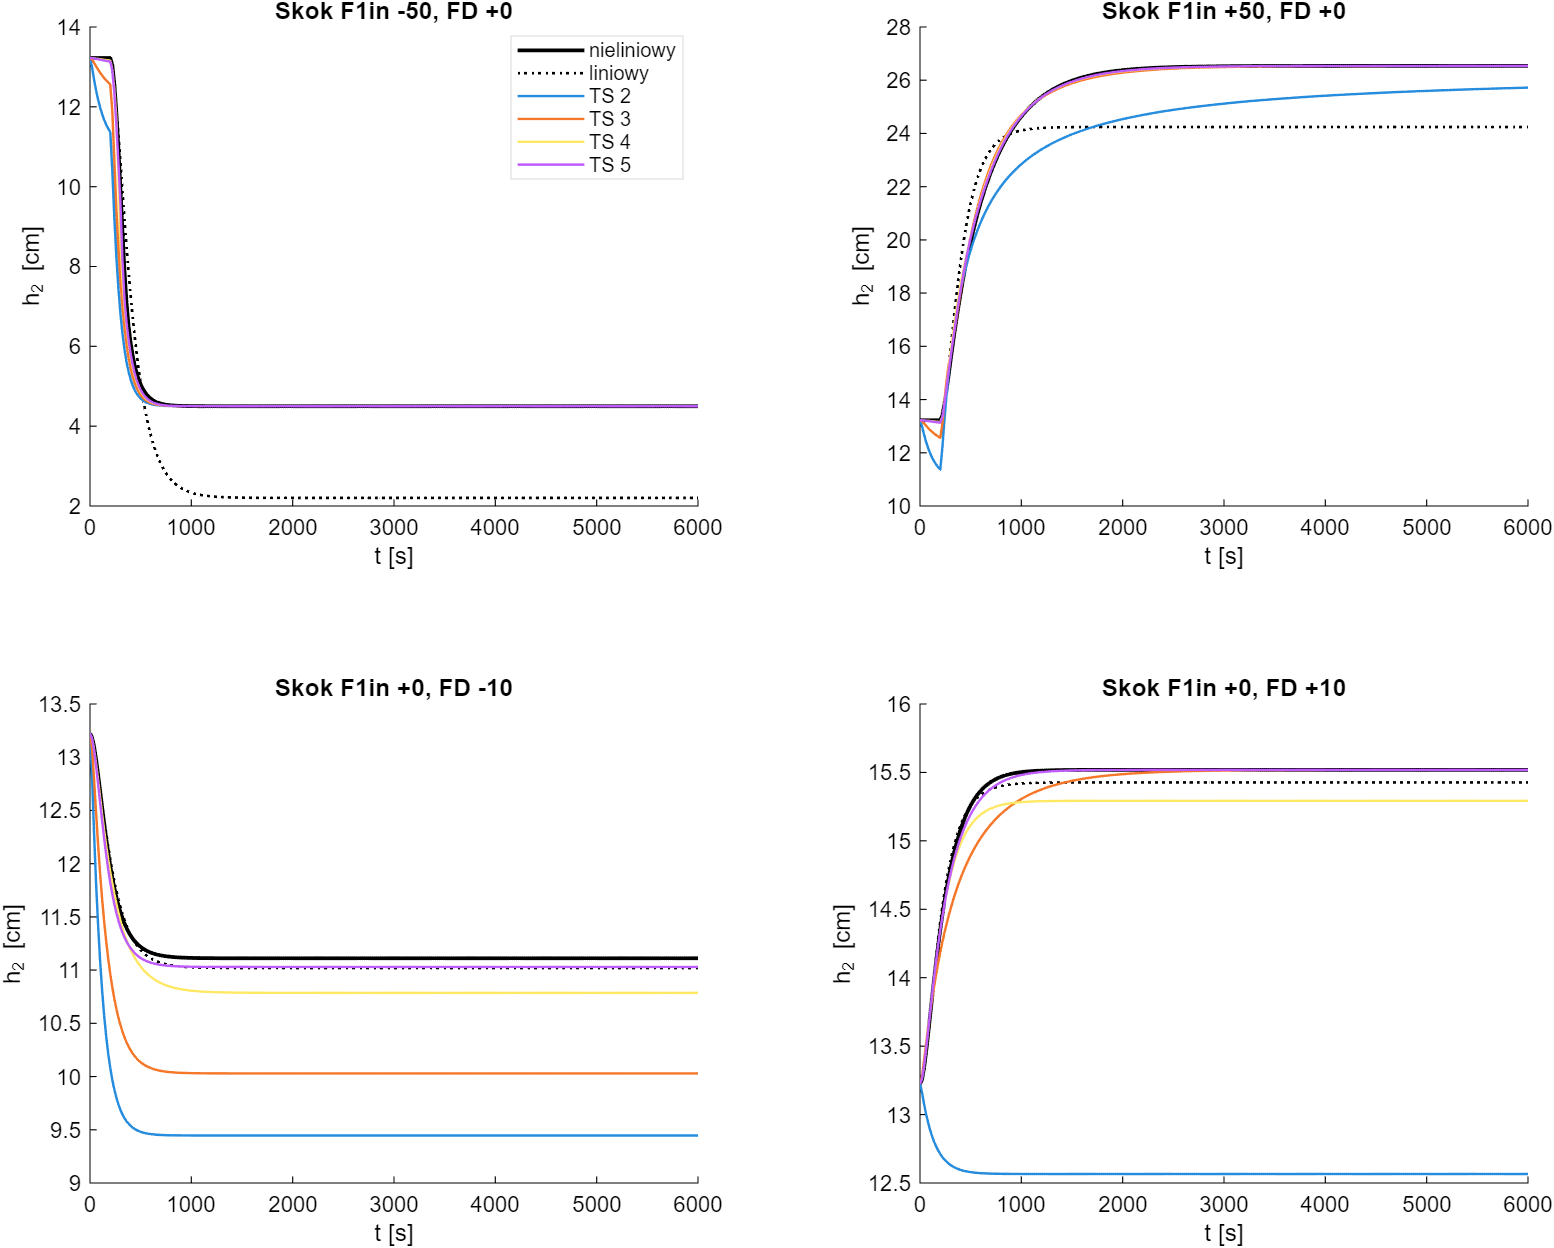
\includegraphics[width=\textwidth]{rysunki/czesc2/modele_2_5.png}
\caption{Odpowiedzi obiektu nieliniowego, modelu liniowego i modeli TS z 2--5 regułami.}
\label{fig:ts-models}
\end{figure}

\section{Strojenie funkcji przynależności modelu}
W modelu pięcioregułowym przesuwano trzy wewnętrzne węzły co 1~cm w zakresie $\pm2\ \mathrm{cm}$ przy stałych końcach przedziału i stałych następnikach. Węzły przed i po strojeniu wynoszą:
\begin{align*}
c_{\mathrm{przed}}&=[\num{4.500},\num{10.009},\num{15.519},\num{21.029},\num{26.538}]\ \mathrm{cm},\\
c_{\mathrm{po}}&=[\num{4.500},\num{8.009},\num{13.519},\num{19.029},\num{26.538}]\ \mathrm{cm}.
\end{align*}
Przesunięcie w stronę mniejszych poziomów poprawiło odwzorowanie w obszarze silniejszej nieliniowości. Łączny RMSE na 12 próbach spadł z \num{0.207} do \num{0.138}~cm (o \num{33.4}\%), a na 4 dodatkowych skokach walidacyjnych ($\Delta\uvar=\pm40$, $\Delta F_D=\pm7\ \jednprzep$) z \num{0.183} do \num{0.153}~cm.

\begin{figure}[H]
\centering
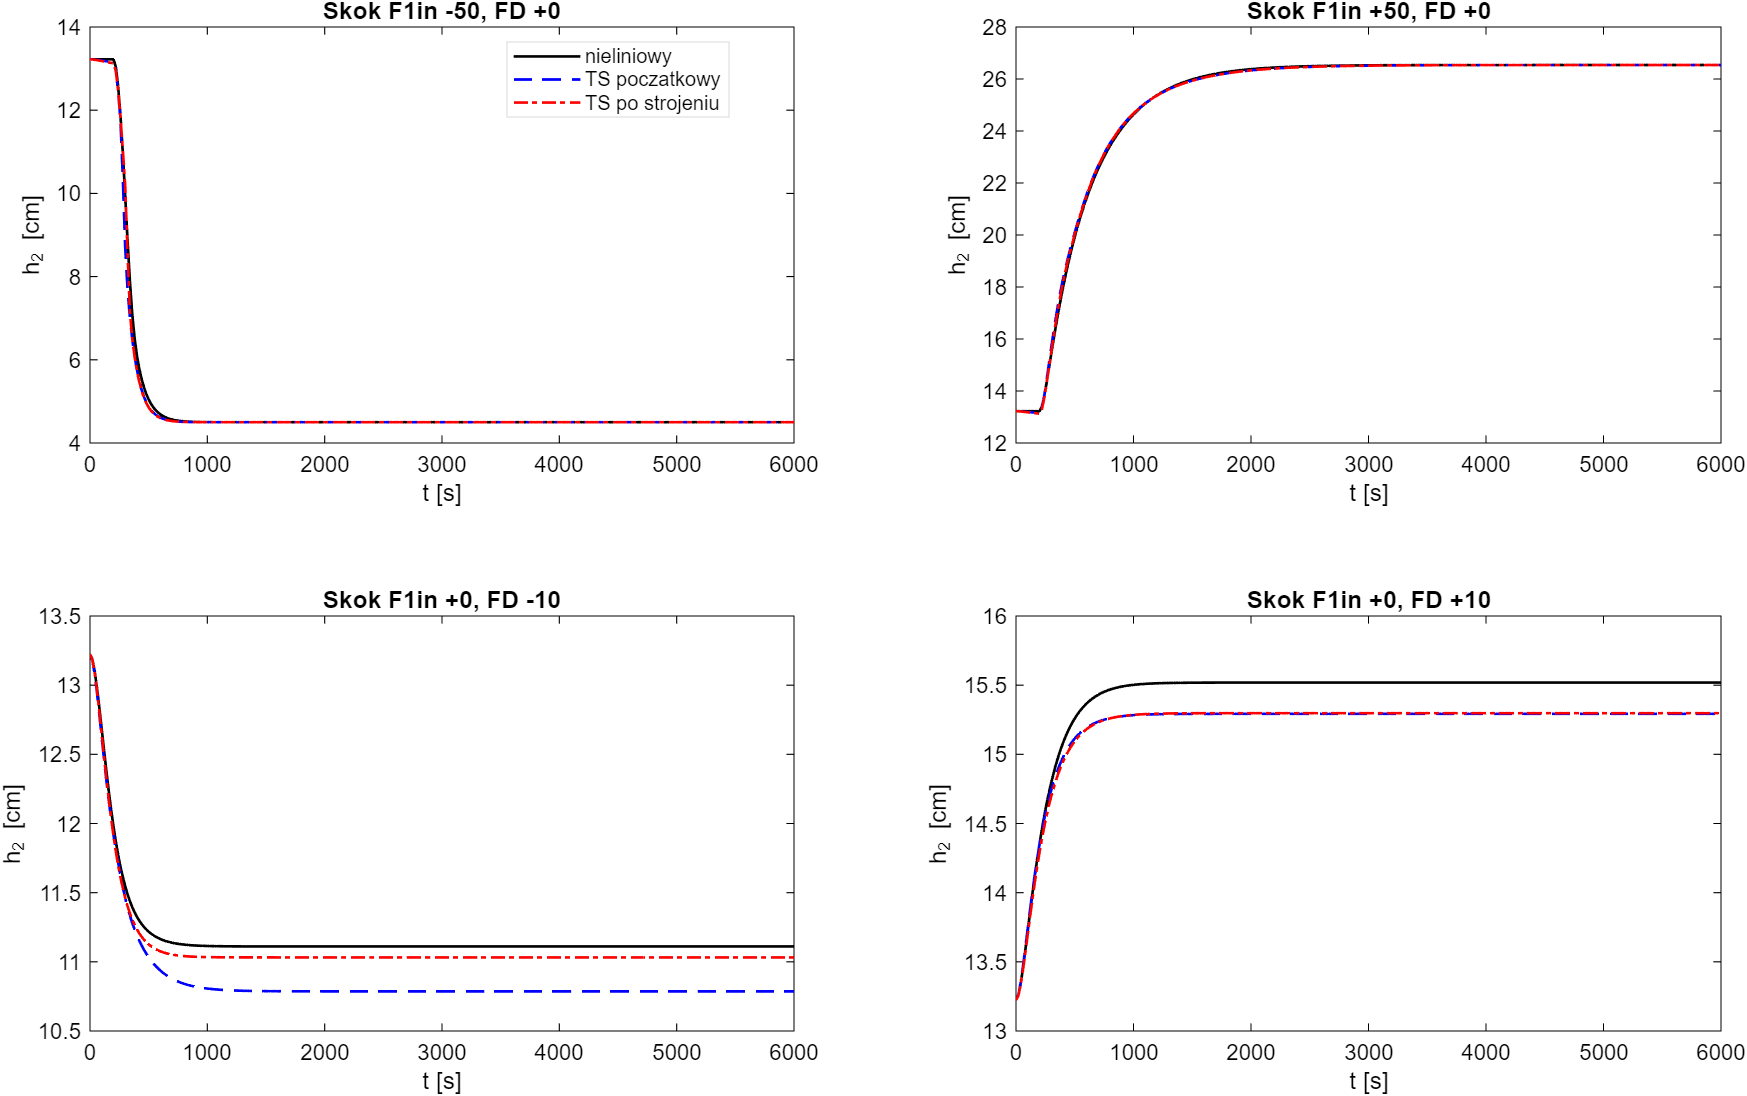
\includegraphics[width=0.95\textwidth]{rysunki/czesc2/porownanie_modeli_TS.png}
\caption{Model pięcioregułowy przed i po strojeniu funkcji przynależności.}
\label{fig:ts-tuned}
\end{figure}

\chapter{Analityczny rozmyty regulator predykcyjny (PDC)}
\section{Algorytm rozmytego DMC i ograniczenia}
Zgodnie z podejściem PDC (materiały wykładowe \emph{Regulatory rozmyte}, s.~148--149, wzory (4.72)--(4.75)) dla każdego z pięciu modeli lokalnych wyznaczono analityczny regulator DMC z odpowiedzi skokowej $s^{(i)}$. Zachowano nastawy z części~1: $D=250$, $N=50$, $N_u=10$, $\lambda=\num{0.05}$, $T_s=20\ \mathrm{s}$.

Dla $i$-tej reguły pierwszy wiersz $k_{1,i}^{\mathsf T}$ macierzy $K_i=(M_i^{\mathsf T}M_i+\lambda I)^{-1}M_i^{\mathsf T}$ wyznacza lokalny przyrost sterowania, a wypadkowy ruch rzutowany jest na ograniczenia:
\begin{align}
 Y_i^0(k)&=y(k)\mathbf 1+M_i^P\Delta U^P(k),\qquad
 \Delta u_i(k)=k_{1,i}^{\mathsf T}\bigl(Y_{\mathrm{zad}}(k)-Y_i^0(k)\bigr),\\
 \Delta u^*(k)&=\sum_{i=1}^5\widetilde w_i\bigl(y(k)\bigr)\,\Delta u_i(k),\\
 L(k)&=\max\bigl(-\Delta u_{\max},\,u_{\min}-u(k-1)\bigr),\qquad
 H(k)=\min\bigl(\Delta u_{\max},\,u_{\max}-u(k-1)\bigr),\\
 \Delta u(k)&=\min\bigl\{H(k),\,\max[L(k),\,\Delta u^*(k)]\bigr\}.
\end{align}
Przyjęto ograniczenia $0\leq\uvar\leq200\ \jednprzep$ i $|\Delta\uvar|\leq15\ \jednprzep$ na próbkę. Początkowe funkcje przynależności regulatora są takie same jak w dostrojonym modelu obiektu. Do porównania zestawiono nieograniczony DMC z części~1 oraz ten sam liniowy DMC z ograniczeniami.

\section{Porównanie układów i strojenie PDC}
Testy wykonano na tej samej osi czasu co w części~1: skok zadania w 400~s, skok $F_D$ w 3800~s, koniec w 8000~s. IAE liczono osobno dla zadania (400--3780~s) i zakłócenia (3800--8000~s).

Strojenie regulatora polegało na zmianie wyłącznie wag przełączania ($\widetilde w_i\propto\mu_i^\gamma$ dla $\gamma$ z zakresu od \num{0.5} do 3) i przesunięciu wewnętrznych węzłów o $\{-2,0,+2\}\ \mathrm{cm}$ przy stałych regulatorach lokalnych. Najmniejszy IAE dało $\gamma=\num{3.0}$ z węzłami $[\num{4.500},\num{10.009},\num{15.519},\num{21.029},\num{26.538}]\ \mathrm{cm}$ (rys.~\ref{fig:ts-controller-mf}).

\begin{figure}[H]
\centering
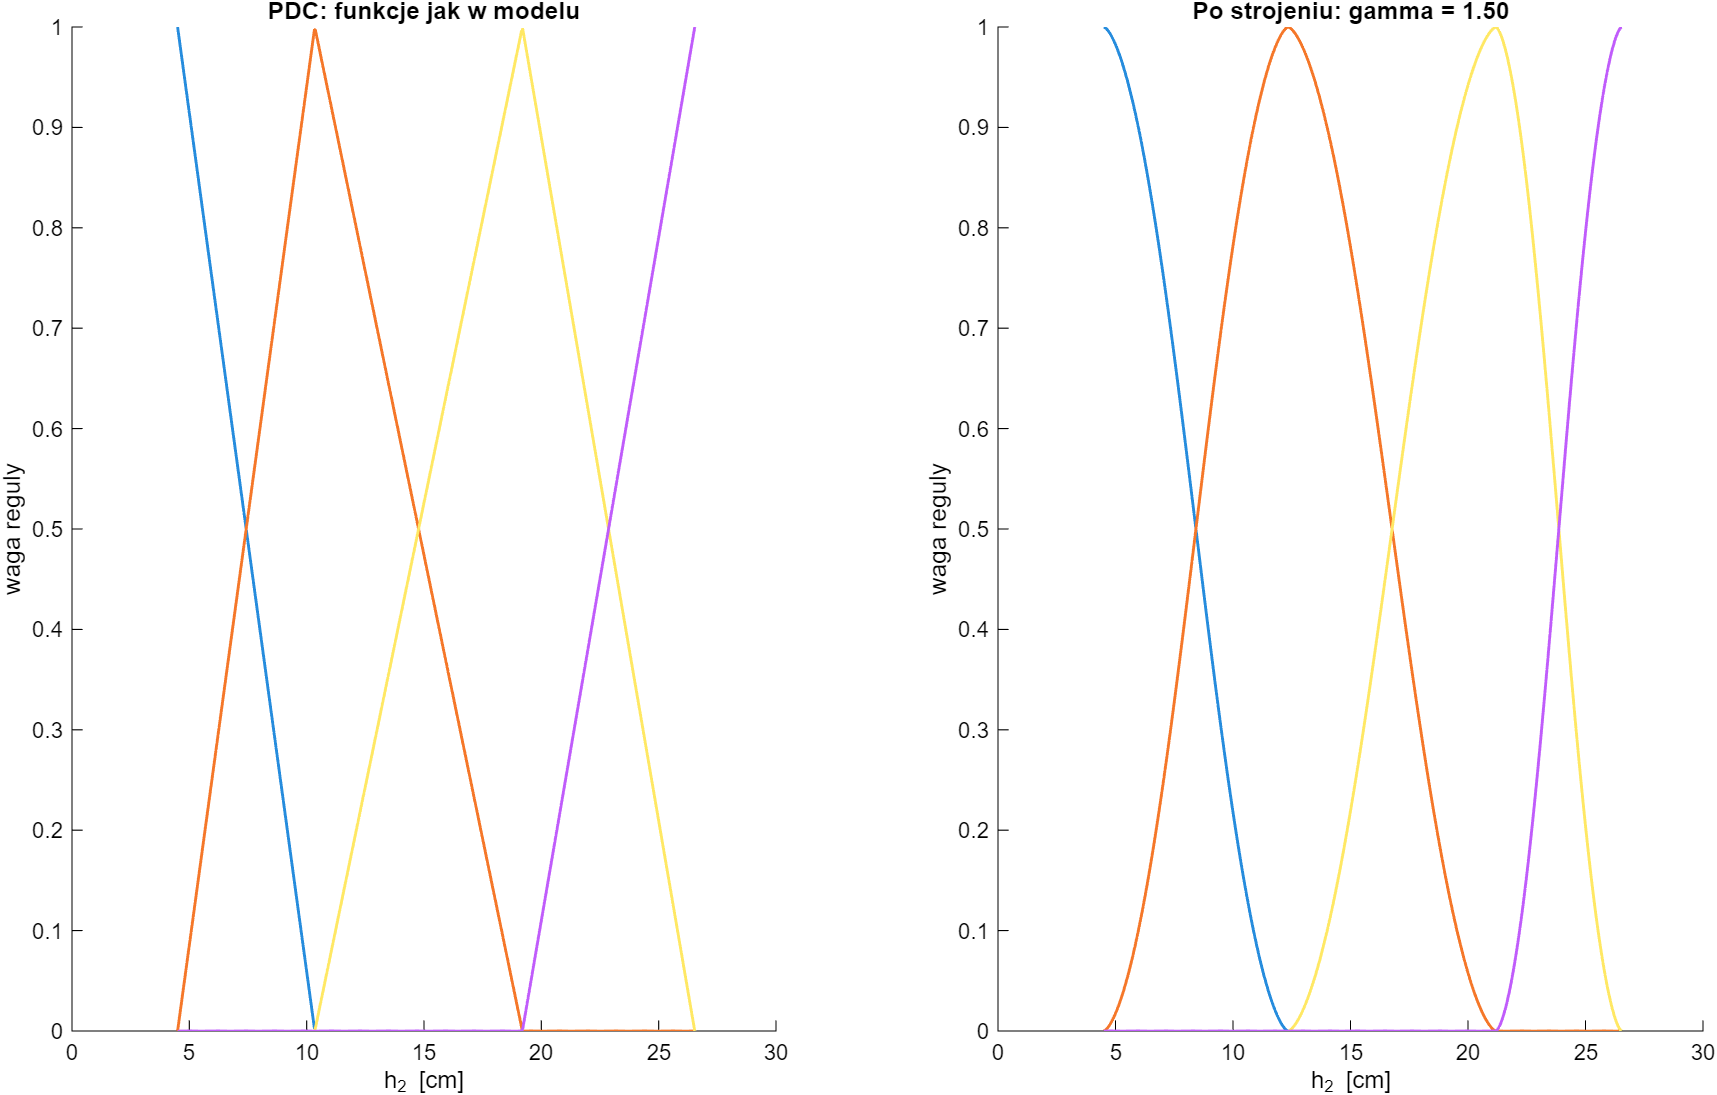
\includegraphics[width=0.94\textwidth]{rysunki/czesc2/strojenie_regulatora.png}
\caption{Funkcje przynależności regulatora PDC przed strojeniem ($\gamma=1$) i po strojeniu ($\gamma=3$).}
\label{fig:ts-controller-mf}
\end{figure}

\begin{table}[H]
\centering
\caption{Suma IAE zadania i zakłócenia w czterech próbach [cm$\cdot$s] ($N=50$, $N_u=10$, $\lambda=\num{0.05}$).}
\small
\begin{tabular}{lrrrr}\toprule
Skoki: zadanie / $F_D$ & DMC cz.~1 & Liniowy ogr. & PDC & PDC strojony\\\midrule
$+2\ \mathrm{cm}/+10\ \jednprzep$ & 1633 & 1633 & 1746 & 1573\\
$+4\ \mathrm{cm}/+20\ \jednprzep$ & 3944 & 3947 & 3809 & 3392\\
$+8\ \mathrm{cm}/+30\ \jednprzep$ & 9483 & 9627 & 7529 & 7001\\
$-8\ \mathrm{cm}/-10\ \jednprzep$ & 4443 & 4579 & 3187 & 3159\\\midrule
Suma & 19503 & 19785 & 16271 & 15125\\\bottomrule
\end{tabular}
\label{tab:ts-control}
\end{table}

Już początkowy PDC obniża sumę IAE o \num{17.8}\% względem ograniczonego DMC liniowego i wyraźnie ogranicza oscylacje przy skokach $\pm8\ \mathrm{cm}$ (rys.~\ref{fig:ts-control}). Po dostrojeniu wag łączny IAE spada o kolejne \num{7.0}\% (do 15\,125~cm$\cdot$s), poprawiając wynik DMC z części~1 o \num{22.5}\% w sumie i w każdej próbie osobno, mimo ograniczenia $|\Delta u|\leq15\ \jednprzep$ (DMC bez ograniczeń wykonywał ruchy do \num{31.12}~$\jednprzep$).

\begin{figure}[H]
\centering
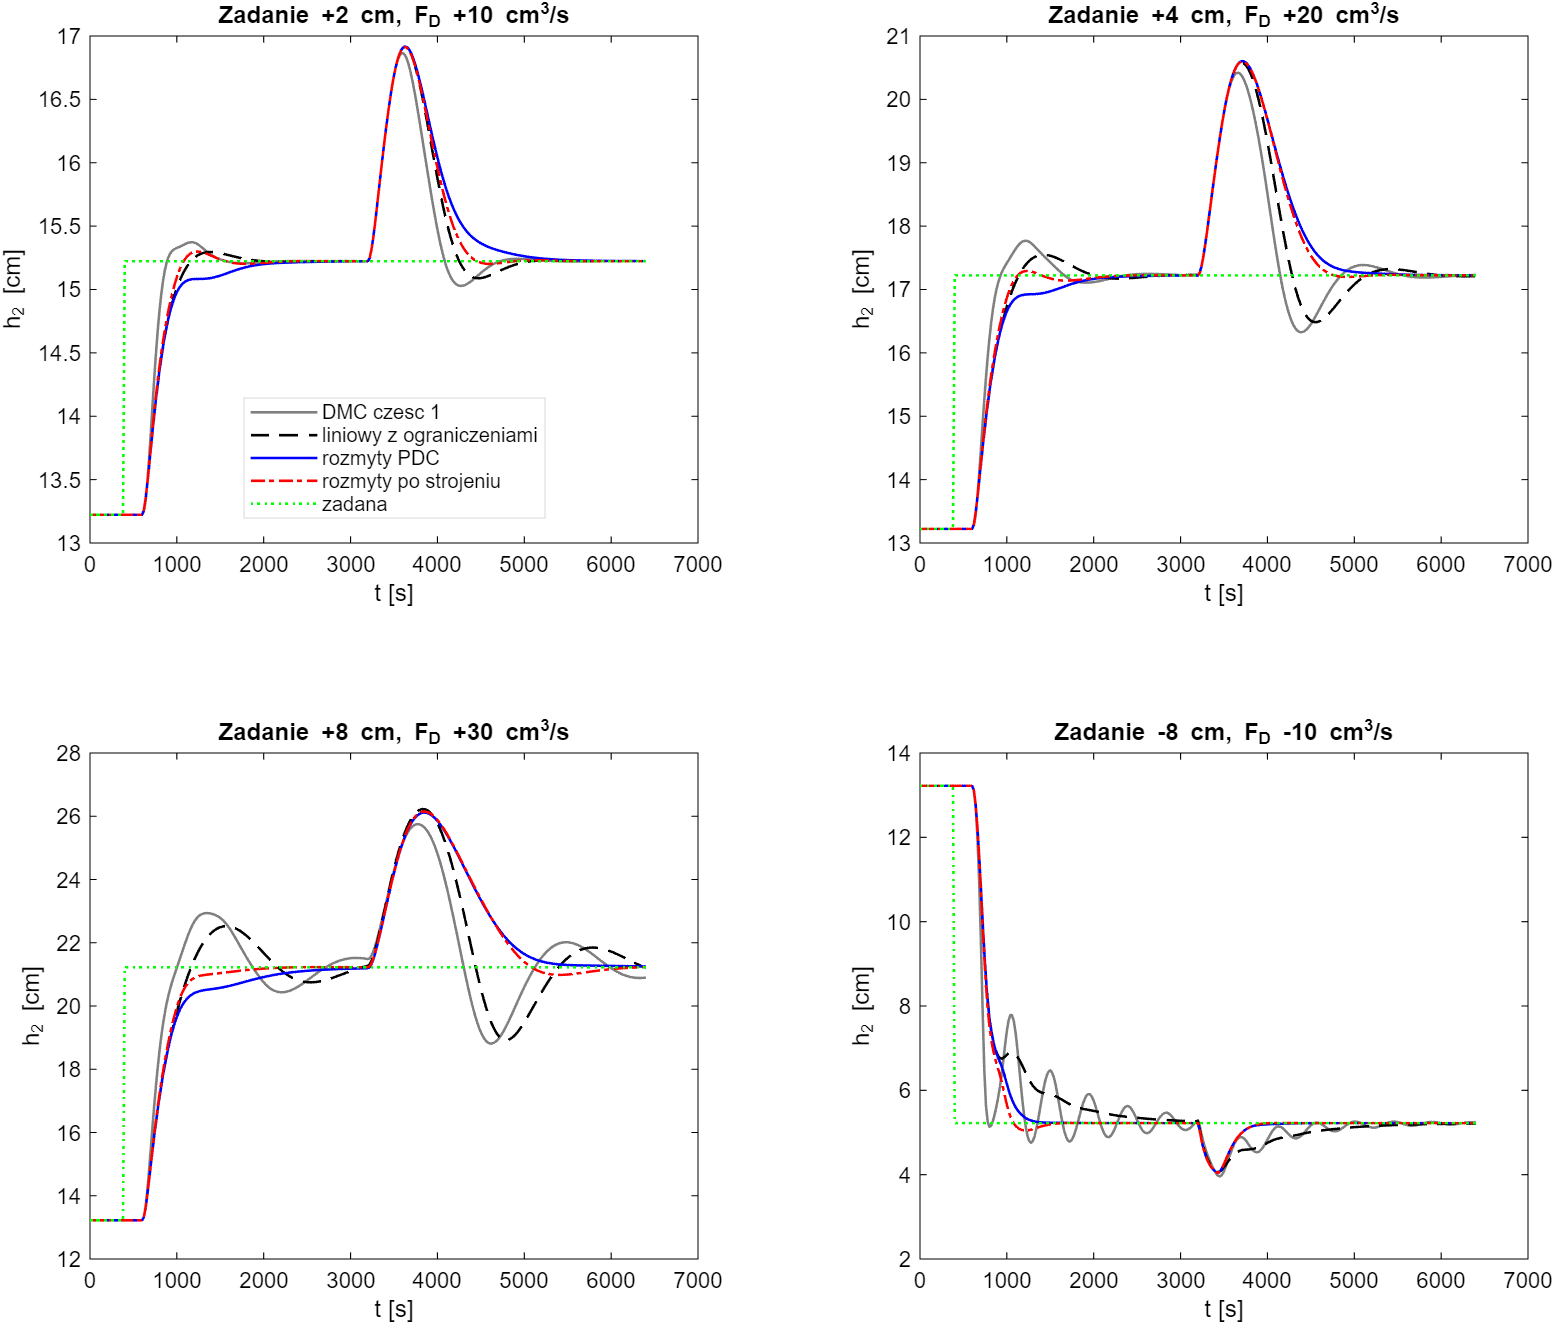
\includegraphics[width=\textwidth]{rysunki/czesc2/regulacja_porownanie.png}
\caption{Przebiegi poziomu $h_2$ dla DMC z części~1, ograniczonego DMC liniowego, PDC oraz PDC po strojeniu.}
\label{fig:ts-control}
\end{figure}

\chapter{Numeryczny rozmyty regulator predykcyjny FGPC--SL}
\section{Algorytm z kolejną linearyzacją i ograniczenia}
W części~3 zaimplementowano numeryczny rozmyty regulator predykcyjny z kolejną linearyzacją w bieżącym punkcie pracy -- algorytm FGPC--SL, zgodnie z materiałami wykładowymi \emph{Regulatory rozmyte}, s.~162--163, wzory (4.103)--(4.105) oraz (4.107). Wykorzystuje on dostrojony pięcioregułowy dyskretny model Takagiego--Sugeno wyznaczony w rozdziale~4.

W każdej chwili próbkowania $k$ regulator wyznacza z bieżącego pomiaru poziomu $y(k)=h_2(k)$ znormalizowane wagi reguł $\widetilde w_i(y(k))$ i uśrednia parametry lokalnych równań różnicowych, uzyskując quasi-liniowy model lokalny (wzór (4.107)):
\begin{align}
 \widetilde b_m(k)&=\sum_{i=1}^5\widetilde w_i\bigl(y(k)\bigr)\,b_{m,i},\qquad
 \widetilde c_m(k)=\sum_{i=1}^5\widetilde w_i\bigl(y(k)\bigr)\,c_{m,i}\quad(m=1,2),\\
 \widetilde a_0(k)&=\sum_{i=1}^5\widetilde w_i\bigl(y(k)\bigr)\,a_{0,i}.
\end{align}
Wagi i parametry tego modelu pozostają zamrożone na całym horyzoncie bieżącej predykcji $p=1,\dots,N$. Z bieżącego równania różnicowego wyznaczana jest odpowiedź skokowa $\widetilde s_p(k)$ (z dziesięcioma początkowymi próbkami zerowymi wynikającymi z opóźnienia $\tau=200\ \mathrm{s}$), która buduje macierz dynamiczną $M_k\in\mathbb R^{N\times N_u}$ o elementach $(M_k)_{pj}=\widetilde s_{p-j+1}(k)$ dla $p\geq j$ i zero dla $p<j$.

Trajektorię swobodną $Y^0(k)=[y^0(k+1|k),\dots,y^0(k+N|k)]^{\mathsf T}$ (dla zerowych przyszłych przyrostów sterowania, tj. $u^0(k+j)=u(k-1)$ dla $j\geq0$) wyznacza się rekurencyjnie z zamrożonego modelu liniowego z addytywną korekcją niezmierzonego zakłócenia i niedokładności modelu $d_k$:
\begin{align}
 y^{\mathrm{mod}}(k)&=\widetilde b_1(k)y(k-1)+\widetilde b_2(k)y(k-2)+\widetilde c_1(k)u(k-11)+\widetilde c_2(k)u(k-12)+\widetilde a_0(k),\\
 d_k&=y(k)-y^{\mathrm{mod}}(k),\\
 y^0(k+p|k)&=\widetilde b_1(k)y^0(k+p-1|k)+\widetilde b_2(k)y^0(k+p-2|k)\nonumber\\
 &\quad+\widetilde c_1(k)u^0(k+p-11)+\widetilde c_2(k)u^0(k+p-12)+\widetilde a_0(k)+d_k,
\end{align}
przy warunkach początkowych $y^0(k|k)=y(k)$ i $y^0(k-1|k)=y(k-1)$. W każdej próbce funkcja \texttt{quadprog} rozwiązuje zadanie optymalizacji kwadratowej (wzory (4.103)--(4.105)):
\begin{align}
 \min_{\Delta U}\quad J&=\lVert Y_{\mathrm{zad}}(k)-Y^0(k)-M_k\Delta U\rVert_2^2
                         +\lambda\lVert\Delta U\rVert_2^2,\\
 -15\mathbf 1\leq\Delta U&\leq15\mathbf 1,\qquad
 0\mathbf 1\leq u(k-1)\mathbf 1+L\Delta U\leq200\mathbf 1,
\end{align}
gdzie $\Delta U=[\Delta u(k),\dots,\Delta u(k+N_u-1)]^{\mathsf T}$, $L$ jest dolnotrójkątną macierzą jedynek sumującą przyrosty, a $Y_{\mathrm{zad}}(k)=h_{2,\mathrm{zad}}(k)\mathbf 1$ bez dodatkowego filtrowania wartości zadanej. Ograniczenia w $\jednprzep$ są identyczne jak w rozdziale~5 i dotyczą całego horyzontu sterowania $N_u$. Do obiektu podawany jest pierwszy obliczony przyrost $\Delta u(k)$, po czym procedura powtarza się w następnej próbce.

\section{Strojenie parametru \texorpdfstring{$\lambda$}{lambda} i porównanie z PDC}
Dla regulatora FGPC--SL przyjęto horyzont predykcji $N=30$ ($600\ \mathrm{s}$, tj. 20 próbek za opóźnieniem transportowym) i horyzont sterowania $N_u=5$. Zgodnie z metodyką strojenia ze skryptu (Przykład~4.18, rys.~4.42--4.43) zbadano wpływ współczynnika kary $\lambda\in\{2;\ 1;\ \num{0.5};\ \num{0.2}\}$ na jakość regulacji i charakter sygnału sterującego. Wszystkie próby przeprowadzono na tym samym obiekcie nieliniowym i osi czasu co w częściach~1 i 2 (skok zadania w $400\ \mathrm{s}$, skok $F_D$ w $3800\ \mathrm{s}$, koniec w $8000\ \mathrm{s}$).

\begin{table}[H]
\centering
\caption{Łączny IAE zadania i zakłócenia w czterech próbach projektowych [cm$\cdot$s]: PDC (cz.~2) oraz FGPC--SL ($N=30$, $N_u=5$).}
\small
\begin{tabular}{lrrrrrr}\toprule
$\Delta h_{2,\mathrm{zad}}$ / $\Delta F_D$ & PDC & PDC str. & SL ($\lambda=2$) & SL ($\lambda=1$) & SL ($\lambda=\num{0.5}$) & SL ($\lambda=\num{0.2}$)\\\midrule
$+2\ \mathrm{cm}/+10\ \jednprzep$ & 1746 & 1573 & 1728 & 1522 & 1403 & 1294\\
$+4\ \mathrm{cm}/+20\ \jednprzep$ & 3809 & 3392 & 3541 & 3098 & 2857 & 2646\\
$+8\ \mathrm{cm}/+30\ \jednprzep$ & 7529 & 7001 & 7066 & 5973 & 5343 & 4899\\
$-8\ \mathrm{cm}/-10\ \jednprzep$ & 3187 & 3159 & 4729 & 4232 & 3957 & 3735\\\midrule
Suma & 16271 & 15125 & 17064 & 14823 & 13561 & 12574\\\bottomrule
\end{tabular}
\label{tab:sl-control}
\end{table}

Tab.~\ref{tab:sl-metrics} rozdziela błędy całkowite po skoku zadania i zakłócenia oraz podaje łączną aktywność sterowania $\sum|\Delta u|$, maksymalny ruch $\max|\Delta u|$, maksymalne cofnięcie na dojściu do zadania, maksymalne przeregulowanie oraz maksymalny uchyb po skoku zakłócenia $F_D$.

\begin{table}[H]
\centering
\caption{Wskaźniki jakości regulacji i aktywności sterowania w czterech próbach projektowych.}
\small
\begin{tabular}{lrrrrrrr}\toprule
Regulator & IAE zad. & IAE zakł. & $\sum|\Delta u|$ & $\max|\Delta u|$ & Cofn. & Przereg. & $\max|e_{F_D}|$\\
 & [cm$\cdot$s] & [cm$\cdot$s] & [$\jednprzep$] & [$\jednprzep$] & [cm] & [cm] & [cm]\\\midrule
PDC                       &  9383 & 6888 & \num{490.6} & \num{15.0} & \num{1.296} & \num{0.232} & \num{4.364}\\
PDC strojony              &  8675 & 6450 & \num{459.6} & \num{15.0} & \num{1.019} & \num{0.473} & \num{4.399}\\
FGPC--SL ($\lambda=2$)    & 11963 & 5102 & \num{221.6} &  \num{5.5} & \num{0.553} & \num{0.506} & \num{3.818}\\
FGPC--SL ($\lambda=1$)    & 10849 & 3975 & \num{272.1} &  \num{8.4} & \num{0.524} & \num{0.497} & \num{3.426}\\
FGPC--SL ($\lambda=0{,}5$)& 10194 & 3366 & \num{325.9} & \num{11.5} & \num{0.504} & \num{0.501} & \num{3.168}\\
FGPC--SL ($\lambda=0{,}2$)&  9633 & 2941 & \num{420.4} & \num{15.0} & \num{1.102} & \num{0.586} & \num{2.958}\\\bottomrule
\end{tabular}
\label{tab:sl-metrics}
\end{table}

Zmniejszanie parametru $\lambda$ przyspiesza śledzenie zadania i znacząco poprawia tłumienie zakłócenia $F_D$ kosztem większej zmienności sterowania (rys.~\ref{fig:sl-tuning}). Jako nastawę kompromisową wybrano $\lambda=\num{0.5}$:
\begin{itemize}
\item względem dostrojonego regulatora PDC łączny wskaźnik IAE spada o \num{10.3}\% (z 15\,125 do 13\,561~cm$\cdot$s), przy czym IAE po zakłóceniu maleje aż o \num{47.8}\% (z 6450 do 3366~cm$\cdot$s), a maksymalny uchyb po skoku $F_D=+30\ \jednprzep$ spada z \num{4.399} do \num{3.168}~cm (o \num{28.0}\%),
\item jednocześnie aktywność sterowania $\sum|\Delta u|$ jest o \num{29.1}\% mniejsza niż w dostrojonym PDC (\num{325.9} wobec \num{459.6}~$\jednprzep$), a największy pojedynczy skok wynosi \num{11.53}~$\jednprzep$ (dopływ pozostaje w bezpiecznym zakresie $\num{55.13}$--$\num{144.87}\ \jednprzep$),
\item dalsze obniżenie kary do $\lambda=\num{0.2}$ redukuje IAE do 12\,574~cm$\cdot$s, lecz nasyca ograniczenie $|\Delta u|\leq15\ \jednprzep$ i ponad dwukrotnie zwiększa odbicie poziomu przy dużym skoku w dół $-8\ \mathrm{cm}$ (cofnięcie wzrasta z \num{0.385} do \num{1.102}~cm, por. rys.~\ref{fig:sl-tuning}).
\end{itemize}
W próbie $-8\ \mathrm{cm}$ wyraźnie ujawnia się ograniczenie metody SL: zamrożenie wag modelu w punkcie startowym $y(k)$ na cały horyzont $N=30$ powoduje niedoszacowanie przyspieszenia spadku poziomu przy małych $h_2$ (gdzie przekrój $3C_2h_2^2$ maleje kilkukrotnie), wskutek czego regulator reaguje z opóźnieniem i wywołuje krótkotrwałe odbicie sterowania oraz poziomu około $t\approx900$--$1100\ \mathrm{s}$ (rys.~\ref{fig:sl-outputs} i \ref{fig:sl-controls}). Czas obliczeń pojedynczego zadania \texttt{quadprog} wynosi średnio poniżej \num{0.4}~ms (maksymalnie \num{4.7}~ms), czyli wielokrotnie mniej niż $T_s=20\ \mathrm{s}$.

\begin{table}[H]
\centering
\caption{Walidacja wariantów FGPC--SL na czterech dodatkowych próbach o przeciwnych znakach wymuszeń [cm$\cdot$s].}
\small
\begin{tabular}{lrrrr}\toprule
$\Delta h_{2,\mathrm{zad}}$ / $\Delta F_D$ & $\lambda=2$ & $\lambda=1$ & $\lambda=\num{0.5}$ & $\lambda=\num{0.2}$\\\midrule
$+3\ \mathrm{cm}/-8\ \jednprzep$  & 2109 & 1870 & 1731 & 1600\\
$-3\ \mathrm{cm}/+12\ \jednprzep$ & 2341 & 2085 & 1933 & 1783\\
$+6\ \mathrm{cm}/-10\ \jednprzep$ & 3987 & 3532 & 3270 & 3049\\
$-6\ \mathrm{cm}/+15\ \jednprzep$ & 4095 & 3665 & 3414 & 3177\\\midrule
Suma IAE (zadanie + zakłócenie)   & 12532 & 11152 & 10348 & 9609\\
Maks. cofnięcie / przereg. [cm]   & \num{0.276} / \num{0.272} & \num{0.275} / \num{0.273} & \num{0.286} / \num{0.284} & \num{0.693} / \num{0.350}\\\bottomrule
\end{tabular}
\label{tab:sl-validation}
\end{table}

Cztery próby walidacyjne o pośrednich amplitudach i przeciwnych znakach skoku zadania oraz zakłócenia (tab.~\ref{tab:sl-validation}) potwierdzają ten sam kompromis strojenia: wariant $\lambda=\num{0.5}$ osiąga mały łączny IAE (10\,348~cm$\cdot$s) przy niewielkim przeregulowaniu i cofnięciu (poniżej \num{0.29}~cm), podczas gdy dla $\lambda=\num{0.2}$ cofnięcie w próbie $-6\ \mathrm{cm}$ rośnie do \num{0.693}~cm.

\begin{figure}[H]
\centering
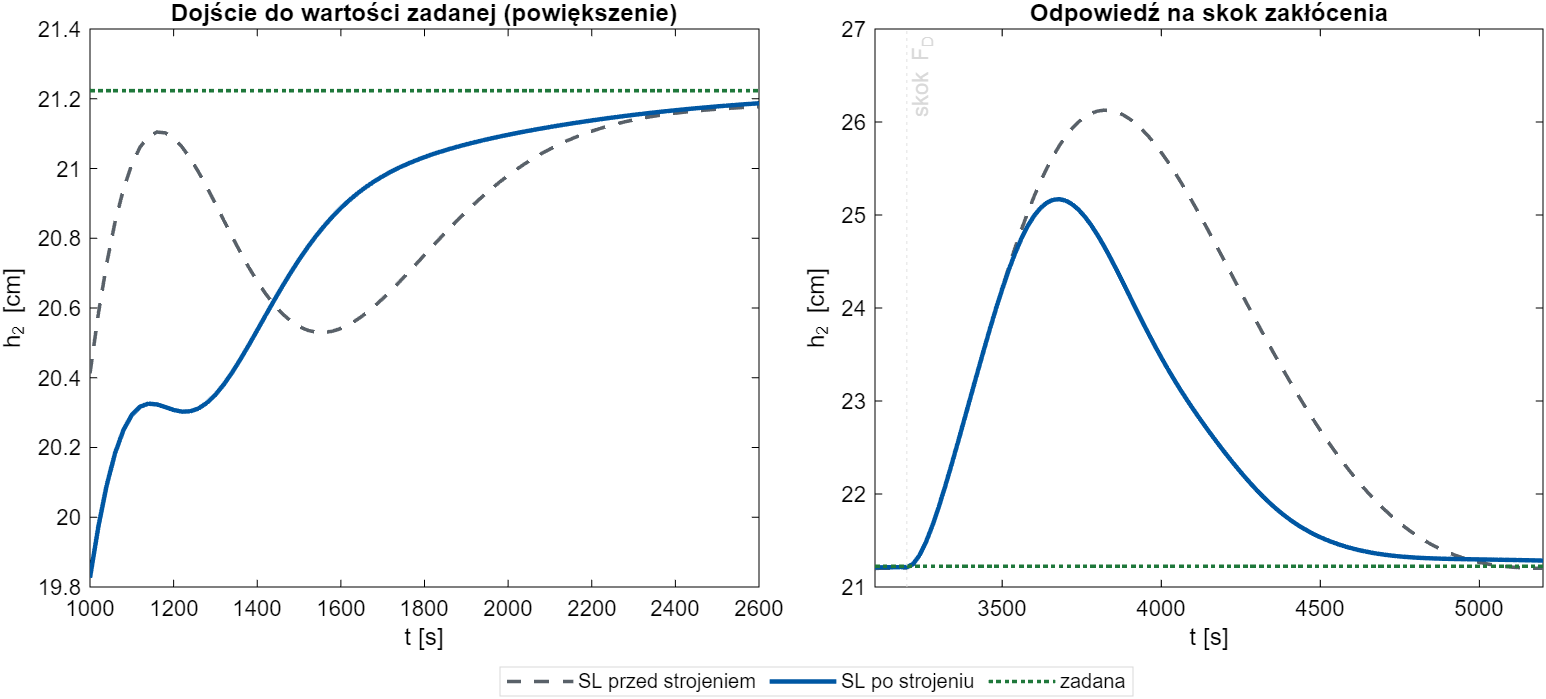
\includegraphics[width=\textwidth]{rysunki/czesc3/strojenie_SL.png}
\caption{Wpływ parametru $\lambda$ w regulatorze FGPC--SL (${N=30}$, ${N_u=5}$) w skrajnych próbach $+8\ \mathrm{cm}$ / $+30\ \jednprzep$ oraz $-8\ \mathrm{cm}$ / $-10\ \jednprzep$.}
\label{fig:sl-tuning}
\end{figure}
\begin{figure}[H]
\centering
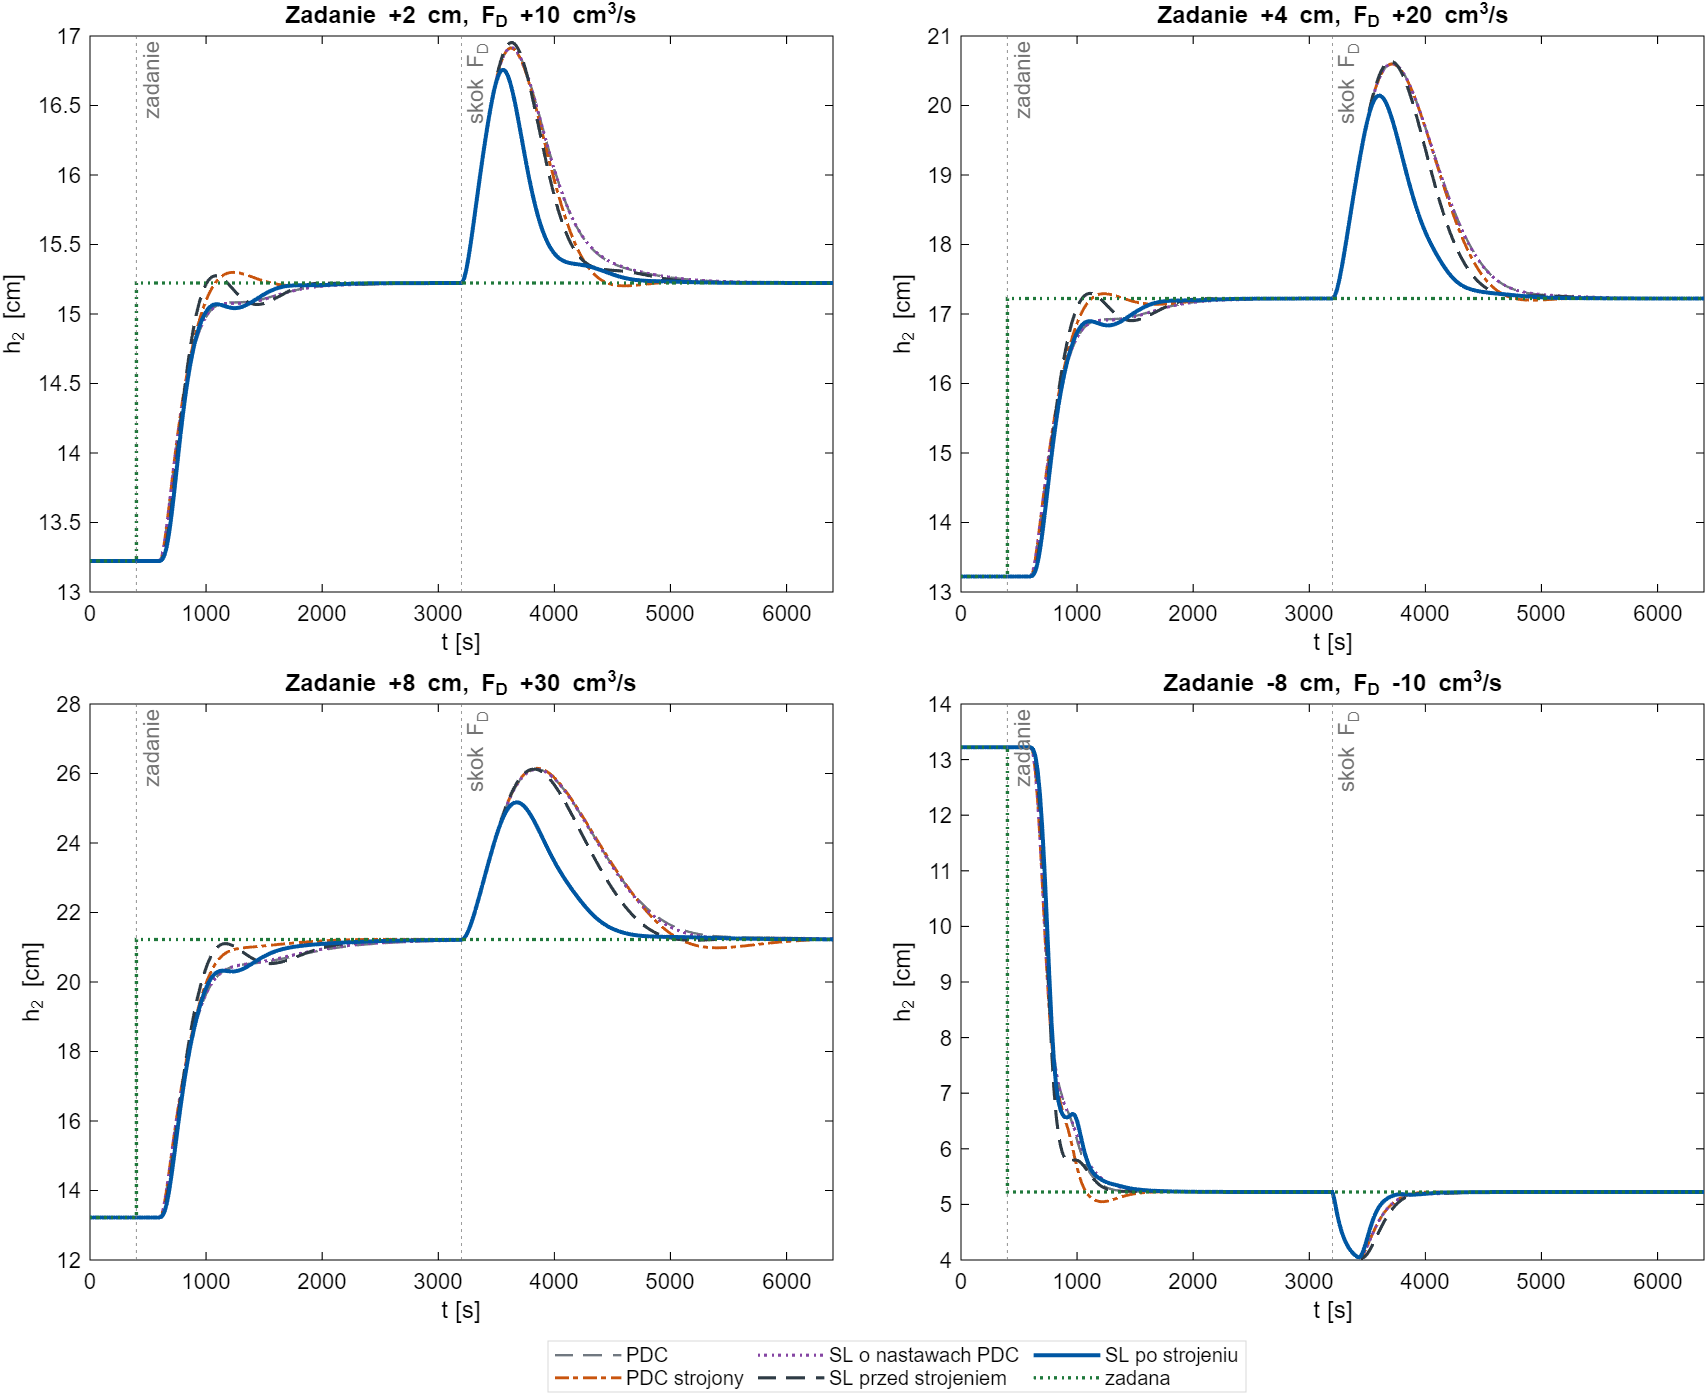
\includegraphics[width=\textwidth]{rysunki/czesc3/porownanie_wyjsc.png}
\caption{Poziom $h_2$ w czterech próbach projektowych: PDC, PDC strojony oraz FGPC--SL (${\lambda=1}$, ${\lambda=\num{0.5}}$ i ${\lambda=\num{0.2}}$).}
\label{fig:sl-outputs}
\end{figure}
\begin{figure}[H]
\centering
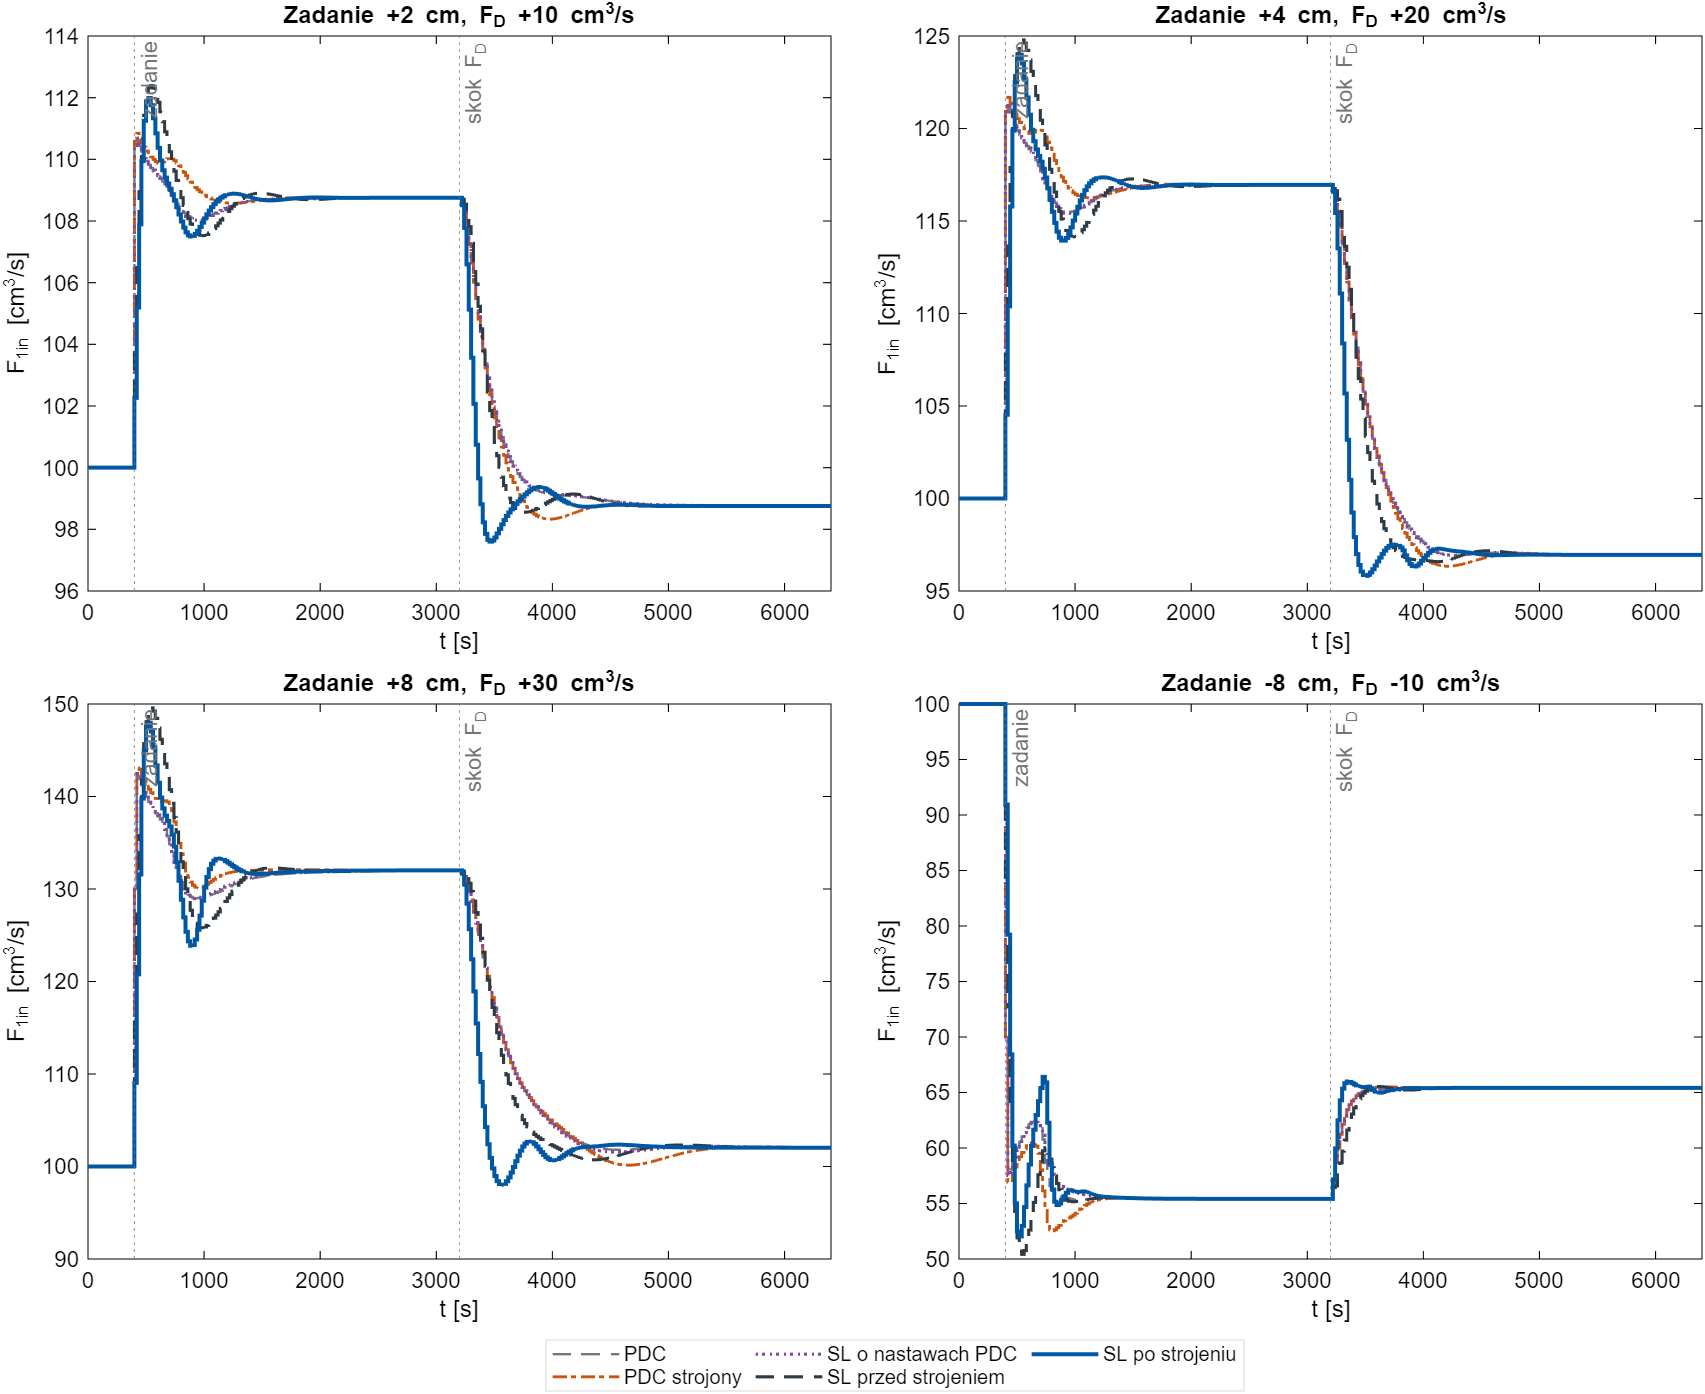
\includegraphics[width=\textwidth]{rysunki/czesc3/porownanie_sterowan.png}
\caption{Dopływ sterujący $\uvar$ dla przebiegów z rys.~\ref{fig:sl-outputs}.}
\label{fig:sl-controls}
\end{figure}

\end{document}
